\documentclass[aspectratio=169,10pt]{beamer}
\usepackage[T1]{fontenc}
\usepackage{lmodern}
\usepackage{amsmath,amssymb,booktabs,array,graphicx,tikz}
\usetikzlibrary{arrows.meta,positioning,calc,shapes.geometric}
\definecolor{forest}{HTML}{145B3D}
\definecolor{deep}{HTML}{103C2B}
\definecolor{leaf}{HTML}{1C8058}
\definecolor{mint}{HTML}{E8F4EC}
\definecolor{sage}{HTML}{A2BAAC}
\definecolor{ink}{HTML}{233B30}
\definecolor{amber}{HTML}{BC8021}
\setbeamercolor{normal text}{fg=ink,bg=white}
\setbeamercolor{frametitle}{fg=white,bg=forest}
\setbeamercolor{title}{fg=white}
\setbeamercolor{structure}{fg=forest}
\setbeamercolor{block title}{fg=white,bg=forest}
\setbeamercolor{block body}{fg=ink,bg=mint}
\setbeamercolor{alerted text}{fg=amber}
\setbeamercolor{itemize item}{fg=leaf}
\setbeamercolor{itemize subitem}{fg=leaf}
\setbeamertemplate{navigation symbols}{}
\setbeamertemplate{headline}{}
\setbeamertemplate{footline}{%
  \leavevmode\hbox{% 
    \begin{beamercolorbox}[wd=.70\paperwidth,ht=.32cm,dp=.14cm,leftskip=.48cm]{normal text}%
    {\color{forest}\fontsize{7.6}{9}\selectfont\bfseries Marcus Maraia \quad | \quad STAT 5200 \quad | \quad November 16, 2026}%
    \end{beamercolorbox}%
    \begin{beamercolorbox}[wd=.30\paperwidth,ht=.32cm,dp=.14cm,rightskip=.44cm plus 1fil]{normal text}%
    \hfill{\color{forest}\fontsize{7.6}{9}\selectfont  \insertframenumber/\inserttotalframenumber}%
    \end{beamercolorbox}}% 
}
\setbeamertemplate{frametitle}{\nointerlineskip\begin{beamercolorbox}[wd=\paperwidth,ht=.79cm,dp=.22cm,leftskip=.45cm]{frametitle}\insertframetitle\end{beamercolorbox}}
\setbeamertemplate{itemize items}[circle]
\setbeamersize{text margin left=.51cm,text margin right=.51cm}
\newcommand{\micro}[1]{{\color{forest}\bfseries\small #1}}
\newcommand{\tinycite}[1]{\par\vspace{.08cm}{\color{gray!85!black}\fontsize{7.4}{9}\selectfont #1}\par}
\newcommand{\figsrc}[1]{\par\vspace{.10cm}{\color{gray!85!black}\fontsize{7.5}{9.2}\selectfont\textbf{Source:} #1}\par}
\newcommand{\takeline}[1]{\begin{beamercolorbox}[wd=\linewidth,sep=7pt,rounded=true]{block body}\color{forest}\bfseries #1\end{beamercolorbox}}
\newcommand{\sr}{\mathrm{SR}}
\title{Can volatility management beat the market?}
\subtitle{Historical alpha, real-time performance, and a preliminary 2019--2025 extension}
\author{Marcus Maraia}
\date{November 16, 2026}
\newcommand{\MKTOrigOne}{0.420}
\newcommand{\MKTManagedOne}{0.513}
\newcommand{\MKTDeltaOne}{+0.092}
\newcommand{\MKTAlpha}{4.607}
\newcommand{\MKTAlphaT}{3.070}
\newcommand{\MKTAlphaP}{0.0021}
\newcommand{\MKTOneP}{0.310}
\newcommand{\MKTFiveP}{0.617}
\newcommand{\MKTOrigFive}{0.458}
\newcommand{\MKTComboFive}{0.415}
\newcommand{\MKTNetSR}{0.432}
\newcommand{\MKTBlockP}{0.169}
\newcommand{\MKTUnmanagedDD}{25.3}
\newcommand{\MKTNetDD}{14.1}
\newcommand{\SMBOrigOne}{0.226}
\newcommand{\SMBManagedOne}{0.076}
\newcommand{\SMBDeltaOne}{-0.150}
\newcommand{\SMBAlpha}{-0.749}
\newcommand{\SMBAlphaT}{-0.865}
\newcommand{\SMBAlphaP}{0.3870}
\newcommand{\SMBOneP}{0.095}
\newcommand{\SMBFiveP}{0.362}
\newcommand{\SMBOrigFive}{0.187}
\newcommand{\SMBComboFive}{0.128}
\newcommand{\SMBNetSR}{-0.654}
\newcommand{\SMBBlockP}{0.104}
\newcommand{\SMBUnmanagedDD}{34.9}
\newcommand{\SMBNetDD}{19.5}
\newcommand{\HMLOrigOne}{0.401}
\newcommand{\HMLManagedOne}{0.367}
\newcommand{\HMLDeltaOne}{-0.033}
\newcommand{\HMLAlpha}{1.753}
\newcommand{\HMLAlphaT}{1.725}
\newcommand{\HMLAlphaP}{0.0846}
\newcommand{\HMLOneP}{0.738}
\newcommand{\HMLFiveP}{0.333}
\newcommand{\HMLOrigFive}{0.442}
\newcommand{\HMLComboFive}{0.375}
\newcommand{\HMLNetSR}{-0.439}
\newcommand{\HMLBlockP}{0.017}
\newcommand{\HMLUnmanagedDD}{39.1}
\newcommand{\HMLNetDD}{10.4}

\begin{document}

\begin{frame}[plain]

\begin{tikzpicture}[remember picture,overlay]
  \fill[deep]
    (current page.south west)
    rectangle (current page.north east);

  \fill[leaf]
    (current page.south west)
    rectangle ([xshift=.075cm]current page.north west);

  % Course identifier
  \node[
    anchor=north west,inner sep=0pt,
    font=\fontsize{9}{12}\selectfont\bfseries,
    text=sage
  ] at ([xshift=.95cm,yshift=-.65cm]current page.north west)
    {STAT 5200 \quad / \quad APPLIED ECONOMETRICS I};

  \draw[sage,opacity=.42,line width=.5pt]
    ([xshift=.95cm,yshift=-1.12cm]current page.north west) --
    ([xshift=-.95cm,yshift=-1.12cm]current page.north east);



  % Main title: independent lines to prevent wrapping
  \node[
    anchor=north west,inner sep=0pt,
    font=\fontsize{27}{33}\selectfont\bfseries,
    text=white
  ] at ([xshift=.95cm,yshift=-2.44cm]current page.north west)
    {Can Volatility Management};

  \node[
    anchor=north west,inner sep=0pt,
    font=\fontsize{27}{33}\selectfont\bfseries,
    text=white
  ] at ([xshift=.95cm,yshift=-3.26cm]current page.north west)
    {Beat the Market?};

  % Accent and subtitle
  \draw[leaf,line width=2pt]
    ([xshift=.95cm,yshift=-4.34cm]current page.north west) --
    ([xshift=2.05cm,yshift=-4.34cm]current page.north west);

  \node[
    anchor=north west,inner sep=0pt,
    font=\fontsize{9.5}{13}\selectfont,
    text=sage
  ] at ([xshift=.95cm,yshift=-4.62cm]current page.north west)
    {Historical Alpha vs. Real-Time Performance};

    \node[
      anchor=north west,
      inner sep=0pt,
      align=left,
      font=\fontsize{9.5}{13}\selectfont,
      text=white!82
    ] at ([xshift=.95cm,yshift=-5.08cm]current page.north west)
      {Replication of \textit{On the Performance of
       Volatility-Managed Portfolios}\\[3pt]
       Cederburg et al.\ (2020)
       \quad $\vert$ \quad
       Preliminary extension: 2019--2025};

  % Footer
  \draw[sage,opacity=.42,line width=.5pt]
    ([xshift=.95cm,yshift=1.27cm]current page.south west) --
    ([xshift=-.95cm,yshift=1.27cm]current page.south east);

  \node[
    anchor=west,inner sep=0pt,
    font=\fontsize{11}{14}\selectfont\bfseries,
    text=white
  ] at ([xshift=.95cm,yshift=.79cm]current page.south west)
    {Marcus Maraia};

  \node[
    anchor=west,inner sep=0pt,
    font=\fontsize{8.5}{11}\selectfont,
    text=sage
  ] at ([xshift=.95cm,yshift=.42cm]current page.south west)
    {University of Pennsylvania};

  \node[
    anchor=east,inner sep=0pt,
    font=\fontsize{9.5}{12}\selectfont,
    text=white
  ] at ([xshift=-.95cm,yshift=.79cm]current page.south east)
    {November 16, 2026};


\end{tikzpicture}
\end{frame}

\begin{frame}{1 \quad The research question}
\begin{columns}[T,onlytextwidth]
\column{.48\textwidth}
\vspace{.2cm}\micro{Economic idea}
\begin{itemize}\setlength{\itemsep}{8pt}
\item Volatile month $\Rightarrow$ reduce next-month factor exposure.
\item Calm month $\Rightarrow$ increase next-month exposure.
\item Goal: improve \textbf{risk-adjusted performance}, not merely reduce volatility.
\end{itemize}
\column{.49\textwidth}
\begin{block}{Three tests of the same idea}
\begin{enumerate}\setlength{\itemsep}{8pt}
\item Stand-alone Sharpe ratio
\item Spanning-regression alpha
\item Real-time portfolio performance
\end{enumerate}
\end{block}
\vspace{.13cm}\micro{Restricted scope}\\[3pt]
MKT (Mkt--RF) \quad SMB (size) \quad HML (value)
\end{columns}
\vfill\takeline{A profitable-looking backtest is not necessarily an implementable investment improvement.}
\end{frame}


\begin{frame}{2 \quad What the published paper contributes}

\begin{columns}[T,onlytextwidth]
\column{.48\textwidth}

\begin{block}{Research lineage}
\textbf{Moreira \& Muir (2017)}\\[4pt]
Positive historical evidence for
volatility-managed portfolios.\\[8pt]

\textbf{Cederburg et al. (2020)}\\[4pt]
Test robustness across
\textbf{103 equity strategies}
and real-time allocation; highlight structural instability.
\end{block}

\hfill
\column{.48\textwidth}

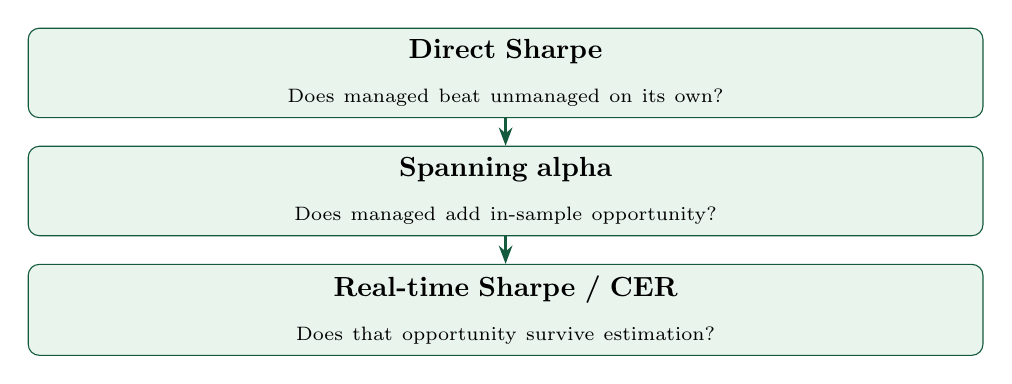
\begin{tikzpicture}[
    every node/.style={align=center},
    node distance=.35cm
]

\node[
    draw=forest,
    rounded corners=4pt,
    fill=mint,
    minimum width=\linewidth,
    minimum height=1.12cm,
    text width=.90\linewidth,
    inner sep=4pt
] (a) {
    {\bfseries Direct Sharpe}\\[4pt]
    {\scriptsize Does managed beat unmanaged on its own?}
};

\node[
    draw=forest,
    rounded corners=4pt,
    fill=mint,
    minimum width=\linewidth,
    minimum height=1.12cm,
    text width=.90\linewidth,
    inner sep=4pt,
    below=of a
] (b) {
    {\bfseries Spanning alpha}\\[4pt]
    {\scriptsize Does managed add in-sample opportunity?}
};

\node[
    draw=forest,
    rounded corners=4pt,
    fill=mint,
    minimum width=\linewidth,
    minimum height=1.12cm,
    text width=.90\linewidth,
    inner sep=4pt,
    below=of b
] (c) {
    {\bfseries Real-time Sharpe / CER}\\[4pt]
    {\scriptsize Does that opportunity survive estimation?}
};

\draw[-{Stealth},forest,thick] (a)--(b);
\draw[-{Stealth},forest,thick] (b)--(c);

\end{tikzpicture}

\end{columns}

\vspace{.18cm}
\takeline{Published takeaway: positive in-sample alphas are not systematic real-time gains.}

\figsrc{Author's conceptual diagram in TikZ, based on Cederburg et al. (2020), Tables 1, 3, 5.}

\end{frame}



\begin{frame}{3 \quad Data and empirical design}


% ============================================
% DATA SOURCE
% ============================================

\micro{Data source and construction}

\vspace{.04cm}

{\small
Kenneth R. French Data Library:
monthly and daily \textbf{Mkt--RF, SMB, and HML}
factor returns. Percentages are converted to decimals
before computing realized variance.
}

\vspace{.04cm}

% ============================================
% HISTORICAL REPLICATION
% ============================================

\begin{block}{
  1 \quad Historical replication
  \hfill
  \small Aug.\ 1926--Dec.\ 2016
}

\small
\textbf{1,085 monthly observations}
\hfill
{\scriptsize Cederburg et al.\ (2020)}

\vspace{.04cm}


\begin{tikzpicture}[x=\linewidth,y=1cm]

  % Proportional observation-count split
  \fill[sage]
    (0,0) rectangle (.1106,.40);

  \fill[forest]
    (.1106,0) rectangle (1,.40);

  % Label within evaluation region
  \node[
    font=\scriptsize\bfseries,
    text=white
  ] at (.555,.20)
    {Expanding-window real-time evaluation};

\end{tikzpicture}

\vspace{.04cm}

\begin{minipage}[t]{.35\linewidth}
{\scriptsize
\textbf{120 months}\\
Initial estimation window
}
\end{minipage}
\hfill
\begin{minipage}[t]{.60\linewidth}
\raggedleft
{\scriptsize
\textbf{965 months}\\
Real-time portfolio evaluation
}
\end{minipage}

\end{block}

\vspace{.04cm}

% ============================================
% OUT-OF-SAMPLE EXTENSION
% ============================================

\begin{block}{
  2 \quad Out-of-sample extension
  \hfill
  \small Jan.\ 2019--Dec.\ 2025
}

\small
\textbf{84 monthly observations}
\hfill
{\scriptsize Author's extension}

\vspace{.04cm}


\begin{tikzpicture}[x=\linewidth,y=1cm]

  % Schematic two-stage process
  \fill[sage]
    (0,0) rectangle (.49,.40);

  \fill[leaf]
    (.51,0) rectangle (1,.40);

  \node[
    font=\scriptsize\bfseries,
    text=deep
  ] at (.245,.20)
    {Calibrate using pre-2019 data};

  \node[
    font=\scriptsize\bfseries,
    text=white
  ] at (.755,.20)
    {Evaluate: 2019--2025};

  \draw[-{Stealth},forest,thick]
    (.49,.20)--(.51,.20);

\end{tikzpicture}

\vspace{.04cm}

{\scriptsize
Scaling fixed using July 1963--Dec.\ 2018 data, following the proposal.\par
Evaluation adds an exposure cap and assumed transaction costs.
}

\end{block}

\vspace{.04cm}

{\color{gray}\fontsize{7.5}{9}\selectfont
\textbf{Diagram note:}
Historical split by observation count; extension schematic, not to calendar scale.
\par}
\end{frame}


\begin{frame}{4 \quad How the managed portfolio is constructed}


\begin{columns}[T,onlytextwidth]

% ============================================
% LEFT COLUMN: METHODOLOGY
% ============================================
\column{.48\textwidth}

\micro{Step 1: Estimate realized variance}

\vspace{.12cm}

\[
\widehat{\sigma}_t^2
=
\frac{22}{J_t}
\sum_{j=1}^{J_t}(f_t^j)^2
\]

\vspace{.04cm}

{\scriptsize
Calculated from daily decimal factor returns
within month $t$, without subtracting the
sample daily mean.
\par}

\vspace{.43cm}

\micro{Step 2: Set next-month exposure}

\vspace{.12cm}

\[
w_{t+1}
=
\frac{c^*}{\widehat{\sigma}_t^2},
\qquad
f_{\sigma,t+1}
=
w_{t+1}f_{t+1}
\]

\vspace{.04cm}

{\scriptsize
Historical $c^*$ uses full-sample normalization;
the extension calibrates $c^*$ before 2019.
\par}

% ============================================
% RIGHT COLUMN: ILLUSTRATION
% ============================================
\column{.48\textwidth}

\micro{Inverse-variance exposure}

\vspace{.12cm}

\begin{center}
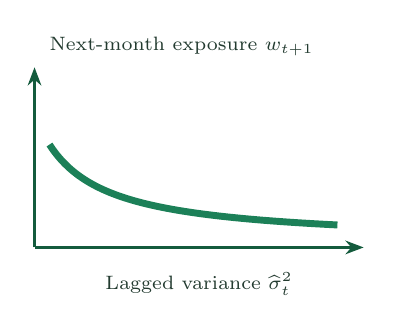
\begin{tikzpicture}[
    x=.95cm,
    y=.88cm,
    >=Stealth
]

% Axes
\draw[->,thick,forest]
    (.45,.45)--(4.85,.45);

\draw[->,thick,forest]
    (.45,.45)--(.45,3.05);

% Inverse-variance curve
\draw[
    leaf,
    line width=2.5pt,
    domain=.65:4.50,
    samples=100,
    smooth
]
    plot (\x,{.52+1.85/(.30+1.55*\x)});

% Y-axis label
\node[
    anchor=south west,
    font=\scriptsize,
    text=ink
] at (.52,3.08)
    {Next-month exposure $w_{t+1}$};

% X-axis label
\node[
    anchor=north,
    font=\scriptsize,
    text=ink
] at (2.65,.23)
    {Lagged variance $\widehat{\sigma}_t^2$};

\end{tikzpicture}
\end{center}

\vspace{.14cm}

{\color{gray!85!black}
\fontsize{7.3}{9}\selectfont
\textbf{Figure source:}
Author's schematic in TikZ, based on
Cederburg et al.\ (2020), Eqs.\ (3)--(4);
not empirical data.
\par}

\end{columns}

\vspace{.20cm}

\takeline{Lag the volatility signal to avoid look-ahead;
cap exposure to limit extreme leverage.}

\end{frame}


\begin{frame}[shrink=10]{5 \quad Table 1: direct Sharpe-ratio replication}
\begin{columns}[T,onlytextwidth]
\column{.72\textwidth}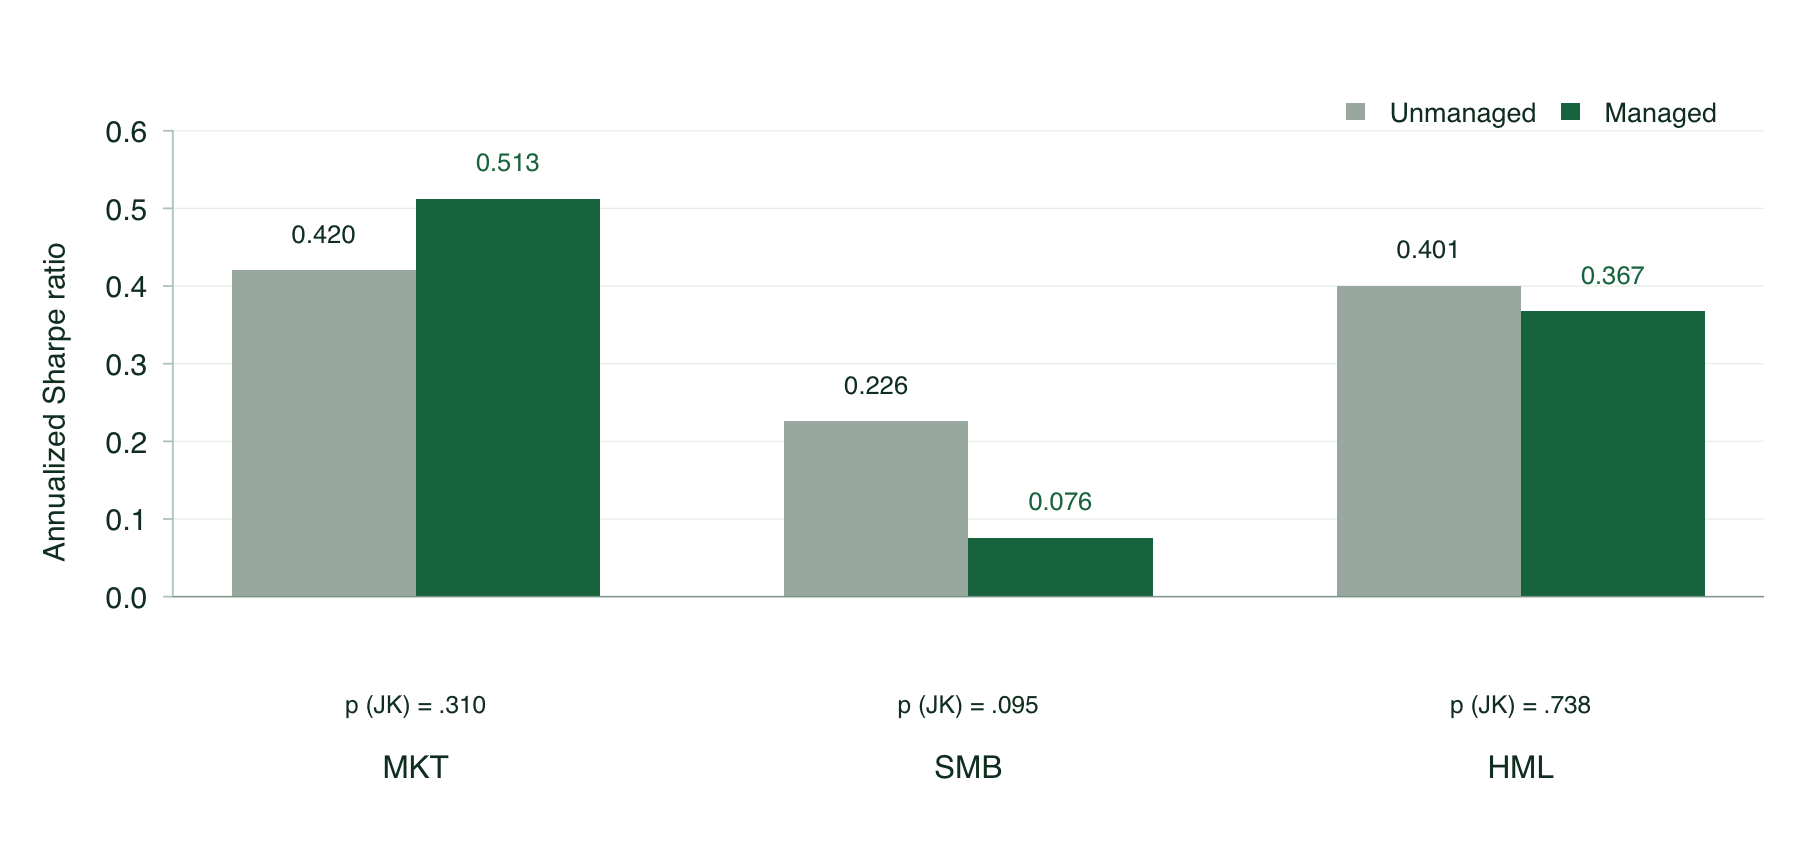
\includegraphics[width=\linewidth]{../../results/figures/01_direct_sharpe.png}
\column{.26\textwidth}
\micro{Computed Sharpe differences}\\[6pt]
MKT: \textbf{\MKTDeltaOne{}}\\[6pt]
SMB: \textbf{\SMBDeltaOne{}}\\[6pt]
HML: \textbf{\HMLDeltaOne{}}\\[13pt]
{\scriptsize Jobson--Korkie test with Memmel correction, as in the paper. All $p>.05$.}
\end{columns}
\vspace{.07cm}
\takeline{Only the market improves in the point estimates; none of the three Sharpe differences is significant at 5\%.}
\figsrc{Author's R chart from computed results using Kenneth R. French data; method: Cederburg et al. (2020), Table 1.}
\end{frame}

\begin{frame}[shrink=5]{6 \quad Table 3: an in-sample alpha opportunity}
\begin{columns}[T,onlytextwidth]
\column{.68\textwidth}
\vspace{.02cm}\micro{OLS spanning regression}
\[f_{\sigma,t}=\alpha+\beta f_t+u_t\]
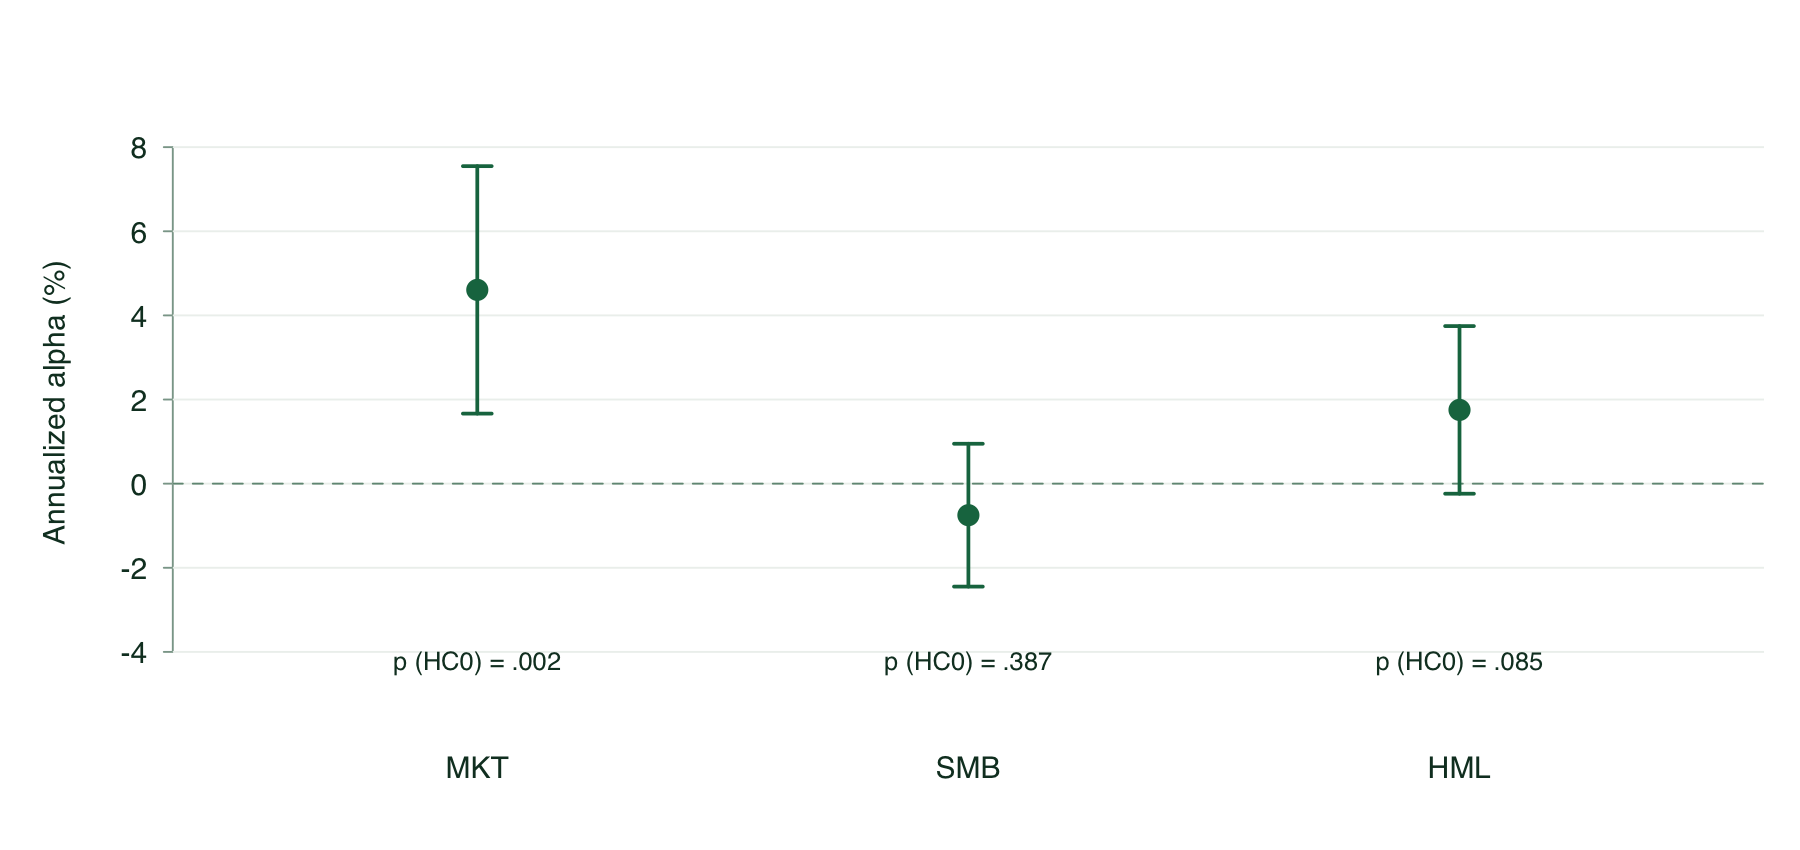
\includegraphics[width=.96\linewidth]{../../results/figures/02_spanning_alpha.png}
\column{.29\textwidth}
\begin{block}{STAT 5200 connection}
\small $y_t=x_t'\theta+u_t$\\[4pt]
\scriptsize OLS projection, \emph{not} causal identification.\\[7pt]
\small $H_0:\alpha=0$\\[4pt]
\scriptsize White HC0 robust $t$ test.\end{block}
\vspace{.12cm}\micro{MKT}\quad $\widehat\alpha=\MKTAlpha{}\%$\\[2pt]
{\scriptsize $t=\MKTAlphaT{}$, $p=\MKTAlphaP{}$}
\end{columns}
\figsrc{Author's R chart from HC0 estimates using Kenneth R. French data; Cederburg et al. (2020), Table 3.}
\vspace{.06cm}\takeline{Market alpha is significant in sample, but alpha is not a promise of real-time investment gains.}
\end{frame}

\begin{frame}[shrink=10]{7 \quad Table 5: what happens in real time?}
\begin{columns}[T,onlytextwidth]
\column{.72\textwidth}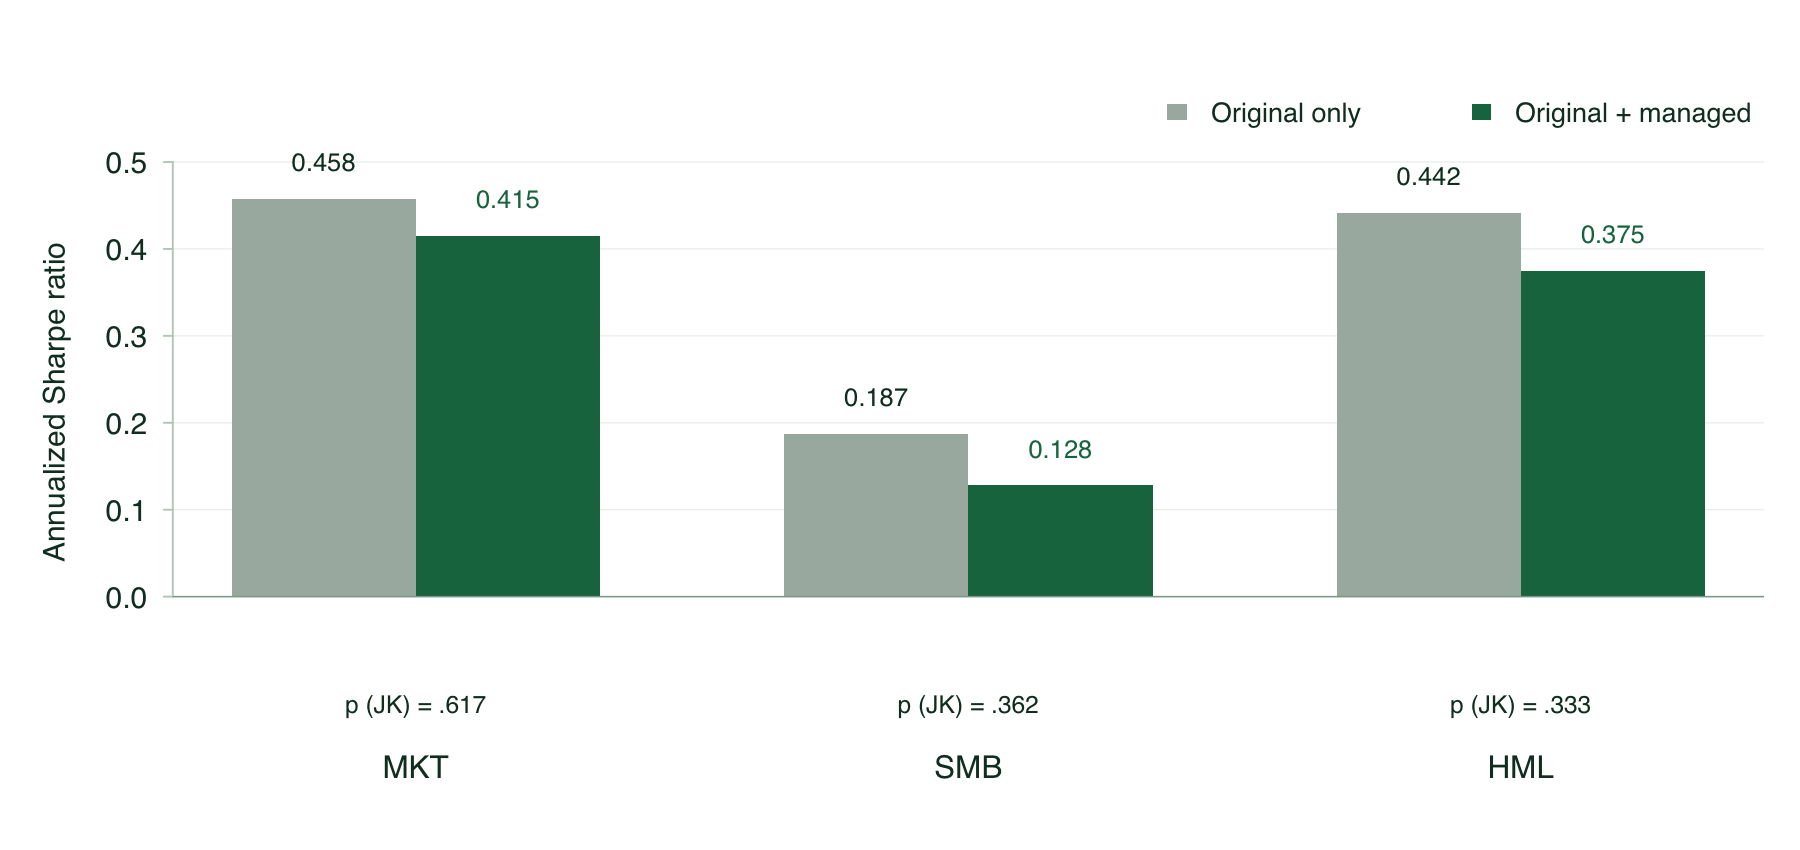
\includegraphics[width=\linewidth]{../../results/figures/03_realtime_sharpe.png}
\column{.26\textwidth}
\micro{Expanding-window design}\\[4pt]
{\scriptsize Train: 120 months. Evaluate: 965 months.\\[4pt]Risk aversion $\gamma=5$; target exposure cap $|y_t|\le5$.}\\[10pt]
\micro{Decision rule}\\[3pt]
{\scriptsize Estimate $\widehat\mu_t$ and $\widehat\Sigma_t$ using returns strictly before month $t$.}
\end{columns}
\vspace{.06cm}\takeline{All three realized Sharpe differences are negative; none is statistically significant at 5\%.}
\figsrc{Author's R chart from portfolio estimates using Kenneth R. French data; Cederburg et al. (2020), Table 5.}
{\color{gray}\fontsize{7.3}{9}\selectfont\textbf{Method caveat:} recursive weights from Eq.\ (15), total exposure from Eq.\ (16), then $|y_t|\le5$ as in Section 4.3.1.}
\end{frame}

\begin{frame}{8 \quad Preliminary extension: 2019--2025 after costs and caps}
\begin{columns}[T,onlytextwidth]
\column{.50\textwidth}
\micro{Net Sharpe ratio}\par\vspace{.10cm}
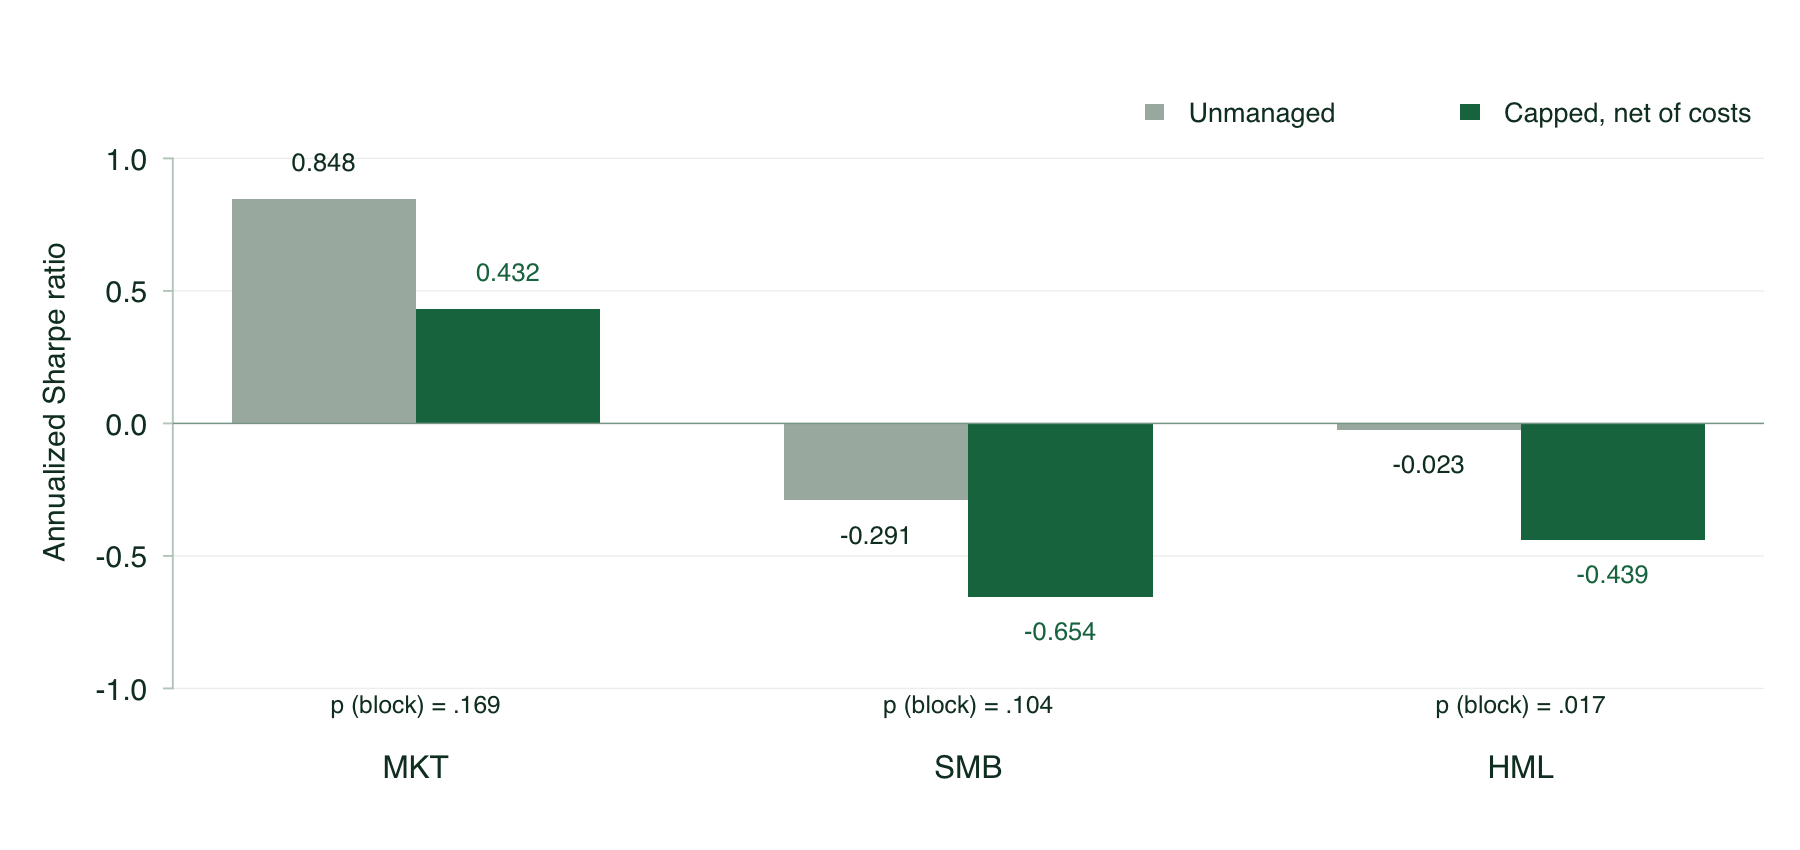
\includegraphics[width=\linewidth]{../../results/figures/04_extension_sharpe.png}
\column{.50\textwidth}
\micro{Max-drawdown magnitude}\par\vspace{.10cm}
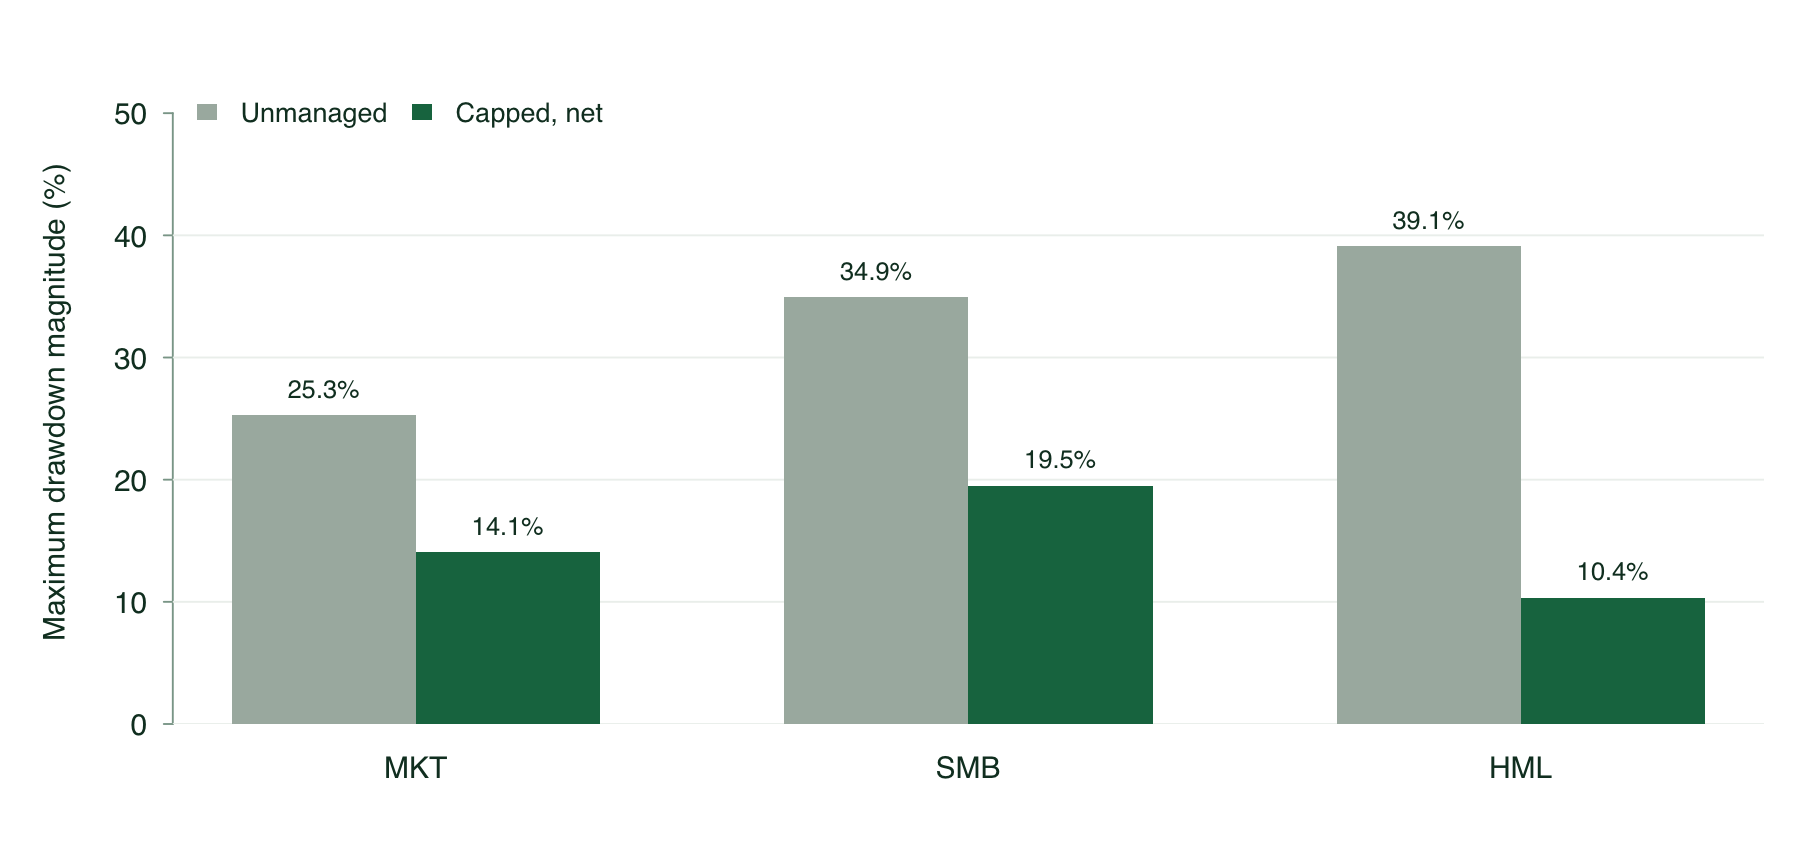
\includegraphics[width=\linewidth]{../../results/figures/05_extension_drawdowns.png}
\end{columns}
\figsrc{Both figures: author's R charts from computed results with Kenneth R. French data, 2019--2025; not published figures.}
\vspace{.04cm}
\begin{beamercolorbox}[wd=\linewidth,sep=5pt]{block body}
\scriptsize \textbf{Rule:} July 1963--Dec.\ 2018 calibration, $|w_t|\le2$; 10 bp per unit of exposure change. \textbf{Inference:} 12-month paired block bootstrap, $B=5{,}000$; HML $p=\HMLBlockP{}$ (exploratory). Drawdowns compound excess returns.
\end{beamercolorbox}
\end{frame}

\begin{frame}{9 \quad What we learned, and what we did not prove}
\begin{columns}[T,onlytextwidth]
\column{.52\textwidth}
\begin{block}{Replication lessons}
\begin{itemize}\setlength{\itemsep}{5pt}
\item Daily return units and one-month timing matter.
\item Ex post scaling $\ne$ deployable calibration.
\item Alpha and Sharpe tests answer \emph{different} hypotheses.
\item Data vintages affect numerical matching.
\end{itemize}
\end{block}
\column{.45\textwidth}
\begin{block}{Boundaries of the evidence}
\begin{itemize}\setlength{\itemsep}{5pt}
\item Three factors, not all 103.
\item 84 recent months; multiple comparisons.
\item Trading costs are factor-level proxies.
\item Historical tests use normal approximations.
\end{itemize}
\end{block}
\end{columns}
\vspace{.16cm}\takeline{Link to my proposal: use this replication as the baseline for testing recent performance after costs and leverage limits.}
\tinycite{Sources: Cederburg et al. (2020); author's R calculations using Kenneth R. French data (November 2026).}
\end{frame}

\appendix
\begin{frame}{Appendix A \quad Historical estimates versus publication}
\small
\begin{center}\begin{tabular}{llrrr}\toprule
Metric & Version & MKT & SMB & HML \\ \midrule
Table 1: original SR & computed & 0.420 & 0.226 & 0.401 \\
Table 1: managed SR & computed & 0.513 & 0.076 & 0.367 \\
Table 1: managed SR & published & 0.51 & 0.08 & 0.38 \\
\midrule
Table 3: alpha (ann. \%) & computed & 4.607 & -0.749 & 1.753 \\
Table 3: alpha (ann. \%) & published & 4.63 & -0.76 & 1.87 \\
\midrule
Table 5: combo SR & computed & 0.415 & 0.128 & 0.375 \\
Table 5: combo SR & published & 0.42 & 0.14 & 0.38 \\
Table 5: original SR & computed & 0.458 & 0.187 & 0.442 \\
Table 5: original SR & published & 0.46 & 0.19 & 0.43 \\
\bottomrule\end{tabular}
\end{center}
\vspace{.16cm}
\tinycite{Published: Cederburg et al. (2020), Tables 1, 3, 5. Computed: author's R analysis using Kenneth R. French data.}
\takeline{Near agreement in values supports the method; it does not prove identical code, vintages, or optimization.}
\end{frame}

\begin{frame}{Appendix B \quad Statistical tests and uncertainty}
\small
\begin{center}\begin{tabular}{lrrr}\toprule
Two-sided $p$-value & MKT & SMB & HML \\ \midrule
Table 1: Sharpe (JK) & 0.310 & 0.095 & 0.738 \\
Table 3: alpha (HC0) & 0.0021 & 0.3870 & 0.0846 \\
Table 5: Sharpe (JK) & 0.617 & 0.362 & 0.333 \\
Table 5: CER (DGU) & 0.811 & 0.258 & 0.679 \\
Extension: Sharpe (block) & 0.169 & 0.104 & 0.017 \\
\bottomrule\end{tabular}
\end{center}
\vspace{.2cm}
\begin{itemize}\setlength{\itemsep}{3pt}
\item Historical Sharpe: Jobson--Korkie/Memmel; CER: DeMiguel et al.\ normal approximation.
\item Alpha: White HC0; heteroskedasticity robust, not serial-correlation robust.
\item Extension only: paired 12-month block bootstrap, $B=5{,}000$; no multiple-testing adjustment.
\end{itemize}
\end{frame}

\end{document}
